% $Id: texintro.tex,v 3:3cfe7538870e 2012/06/08 23:22:24 stanton $
%\documentclass[12pt,twoside]{article}
\documentclass[12pt]{article}

% Standard list of included packages
\usepackage{setspace}           % Allows easy changes to line spacing 
\usepackage{graphicx}           % Allows including of graphics files
\usepackage{amsmath}            % Additional math capabilities
\usepackage{marginnote}         % Used with todonotes package
\usepackage{datetime}           % Allows formatting of date and time
\usdate                         % Use usual LaTeX date layout
\usepackage{enumitem}           % Change formatting of lists
\usepackage{subfigure}          % Create numbered and captioned subfigures
\usepackage{rotating}           % Create landscape tables and figures
\usepackage{hyperref}           % URLS and hyperlinks
\usepackage{float}              % Activate [H] option to place figure HERE
\usepackage[longnamesfirst]{natbib} % Bibliography formatting

% Packages included specifically for this document.
\usepackage{texintro}           % Document-specific definitions
\usepackage{tocvsec2}           % More flexible formatting of table of contents
\usepackage{bibentry}           % Print full citation in text
\usepackage[retainorgcmds]{IEEEtrantools}  % Equation formatting. Option needed to
                                           % allow enumitem to work.
\usepackage{versionPO}          % Include text conditionally

% These next lines allow including or excluding different versions of text
% using versionPO.sty

\includeversion{notes}		% Include notes?
%\excludeversion{notes}
\excludeversion{comment}
\includeversion{links}          % Turn hyperlinks on?
\excludeversion{submit}		% Format for conference submission?
\includeversion{toc}		% Include table of contents?

% Turn off hyperlinking if links is excluded
\iflinks{}{\hypersetup{draft=true}}

% Notes options
\ifnotes{%
\usepackage[margin=1in,paperwidth=10in,right=2.5in]{geometry}%
\usepackage[textwidth=1.4in,shadow,colorinlistoftodos]{todonotes}%
}{%
\usepackage[margin=1in]{geometry}%
\usepackage[disable]{todonotes}%
}

% Allow todonotes inside footnotes without blowing up LaTeX
% Next command works but now notes can overlap. Instead, we'll define 
% a special footnote note command that performs this redefinition.
%\renewcommand{\marginpar}{\marginnote}%

% Save original definition of \marginpar
\let\oldmarginpar\marginpar

% Workaround for todonotes problem with natbib (To Do list title comes out wrong)
\makeatletter\let\chapter\@undefined\makeatother % Undefine \chapter for todonotes

% Define note commands
\newcommand{\smalltodo}[2][] {\todo[caption={#2}, size=\scriptsize, fancyline, #1] {\begin{spacing}{.5}#2\end{spacing}}}
\newcommand{\rhs}[2][]{\smalltodo[color=green!30,#1]{{\bf RS:} #2}}
\newcommand{\rhsnolist}[2][]{\smalltodo[nolist,color=green!30,#1]{{\bf RS:} #2}}
\newcommand{\rhsfn}[2][]{%  To be used in footnotes (and in floats)
\renewcommand{\marginpar}{\marginnote}%
\smalltodo[color=green!30,#1]{{\bf RS:} #2}%
\renewcommand{\marginpar}{\oldmarginpar}}

\newcommand{\textnote}[1]{\ifnotes{{\colorbox{yellow}{{\color{red}#1}}}}{}}

% Number paragraphs and subparagraphs and include them in TOC
\setcounter{tocdepth}{2}

\begin{document}

\nobibliography*                                % Allow use of \bibentry command
\setlist{noitemsep}                             % Reduce space between list items 

% Define commands for title, acknowledgments and abstract. This saves
% typing later as you may want these to appear in different locations
% depending on whether paper is to be processed as a working paper, submission
% to journal, etc.
\newcommand{\tit}{Writing Finance Papers Using \LaTeX}

\newcommand{\ack}{I am grateful to Jennifer Carpenter and Johan Walden for valuable input (even if some of it was inadvertent). I am also grateful to Tobias Oetiker for writing the \texttt{example} environment, which I use liberally in this document. \textnote{INCLUDES NOTES.} \rhsfn[nolist]{I like to have this on the front page to reduce the likelihood that the paper will go back to the journal complete with all my insulting comments about the referee.}}

\newcommand{\abs}{
This document provides some recommendations for efficiently writing finance papers using \LaTeX\ and related tools, based on techniques that have made me more productive over the years. It also contains the necessary \LaTeX\ style files and  Bib\TeX\ format files (along with sample paper outlines) for making your paper and bibliography match the formats required by the \emph{Journal of Finance}, \emph{Journal of Financial Economics}, and \emph{Review of Financial Studies}. The source file, \texttt{texintro.tex}, and various additional included files are important parts of this document.
}

\title{\tit\ifsubmit{}{\thanks{\ack}} \rhs[nolist]{Notes like this appear throughout the document and are created using the \texttt{todonotes} package (see Section~\ref{sec:todo}).}}

\ifsubmit{}{\author{Richard Stanton\thanks{Haas School of Business,
    U.C.\ Berkeley, 545 Student Services Building \#1900, Berkeley, CA
    94720-1900, phone: 510-642-7382, fax: 510-643-1412, e-mail:
    stanton@haas.berkeley.edu.}}}

% Printing time as well as date helps keep track of different revisions 
% during the day.
\date{\ifsubmit{}{\today, \currenttime \rhs[nolist]{Including the current time helps to locate the latest printout in that huge pile on your desk when you create many versions of a paper during the day (see \texttt{datetime} package, Section~\ref{sec:datetime}).}}}

%If you just want the date, but not the time
%\date{\today}
%\date{June 21, 2012}

\maketitle
\thispagestyle{empty}

\begin{abstract}
  \abs
\end{abstract}

% Move to next page. If twoside option is selected above, next page will start 
% on right-hand side.
\cleardoublepage

% Select spacing
\onehalfspacing

\setcounter{page}{1}

% Print table of contents (if desired)
\begin{toc}
\begin{singlespacing}
\tableofcontents
\end{singlespacing}
\clearpage
\end{toc}

\section{Introduction}

\LaTeX\ is a document typesetting system, based on Knuth's program \TeX{} \citep[see][]{Knuth:84}\rhs[nolist]{Section~\ref{sec:bib} deals with creating citations and bibliographies. Note that this link is live and clickable (see \texttt{hyperref} package, Section~\ref{sec:hyperref}).}, which makes it relatively simple to produce papers with high-quality equations and error-free cross-references to equations, tables, and figures, and to handle creation and formatting of bibliographies and citations.\footnote{Plenty of people use word processors for writing papers instead. This makes no sense to me, but rather than engage in a debate, I'll just note that if you use Word this document is probably not going to be very useful to you.}
This document is not a comprehensive overview of \LaTeX. It is, rather, a collection of suggestions for tools and techniques that make me more productive when I write papers, along with some instructions and sample files for formatting your papers to match the requirements of the \emph{Journal of Finance}, \emph{Journal of Financial Economics}, and \emph{Review of Financial Studies}.

If you're starting from scratch, 
one very popular reference, free to download, is the ``Not So Short Introduction to \LaTeXe''  \citep{OetikerPartlHynaSchlegl:11}.  There are also some excellent books on \LaTeX. Standard references include \cite{Lamport:94}, written by the original author of \LaTeX; \cite{KopkaDaly:03}, a more recent, popular introductory text; and \cite{MittelbachGoossensBraamsCarlisleRowley:04}, an excellent reference on both \LaTeX\ itself and many of the additional packages that have been created since \LaTeX\ was created (the authors of this book are some of the main developers of \LaTeX).\footnote{I own and refer to all of these books, especially \cite{MittelbachGoossensBraamsCarlisleRowley:04}, and I originally learned \LaTeX\ from \cite{Lamport:94}. You can also find other references at \url{http://www.ctan.org/starter.html}. However, I find that nowadays I use Google more than any other reference.}

Creation of a document using \LaTeX\ is a two-step process:
\begin{enumerate}
\item Create a \LaTeX\ source file, usually with the extension \verb|.tex|, containing your text plus commands that tell \LaTeX\ how to format your document.\rhs[nolist]{By default, \LaTeX\ inserts more space between list items than this (see \texttt{enumitem} package, Section~\ref{sec:enumitem}).}\footnote{For example, the source for this document is called \texttt{texintro.tex}. Unlike word-processor files, \LaTeX{} files are plain text, with no special control codes. This makes them easily portable from one machine (or architecture or OS) to another, easy to view using any plain-text file viewer, and also means that you stand a decent chance of being able to rescue a lot of your material if the file accidentally gets corrupted, say by a misbehaving word processor or a disk failure. Not that files get corrupted all that often, of course, but just in case, it's nice to know. This also makes it easy to keep track of your work using a Version Control System (see Section~\ref{sec:VCS}).} 
\item Process the .tex file to create the final PDF file.\footnote{Before PDF became standard, it was usual for the .tex file to be processed to a .dvi (\textbf{D}e\textbf{v}ice \textbf{I}ndependent) file, which was then further processed to a printable format using a printer-specific executable (e.g., \texttt{dvips} for Postscript or \texttt{dvilj} for an HP Laserjet). To create a PDF file, you would 1) run \texttt{latex} to create a .dvi file, 2) run \texttt{dvips} to convert the .dvi file into a Postscript file, and 3) run Adobe Distiller (or Ghostscript) to convert the PS file to PDF. Nowadays this is usually done in one step (using the \texttt{pdflatex} program behind the scenes). Yes, I know you still insist on using \texttt{dvips}, Johan, though I have no idea why\ldots.}
\end{enumerate}
For example, here is an extremely simple \LaTeX{} file (the text after ``\%'' on each line is just a comment; it is ignored by \LaTeX):
\begin{verbatim}
\documentclass{article}              % Tell LaTeX to use the "article" style
\begin{document}                     % Document starts here
This is my first paper.              % Text
\end{document}                       % Document ends here
\end{verbatim}
If you process this file using  \LaTeX, it produces the following PDF file:\footnote{There's also a page number at the bottom of the page, which I've omitted to save space.} 

\vspace{0.3in}
\centerline{\frame{
\includegraphics[trim=0in 8.5in 0in 1.5in, clip=true, width=6.5in]{test}}}

\rhs[inline]{Describe what the paper contains.}


\section{Installing \LaTeX{}}

Writing papers using \LaTeX\ requires, in principle, three separate pieces of software:
\begin{enumerate}
\item A text editor to edit the .tex source file.
\item \TeX/\LaTeX\ software to process your source file and create the final PDF file.
\item A PDF viewer so you can see the output.
\end{enumerate}
While you can install three separate pieces of software, it is much simpler to use a \LaTeX\ installation that comes with a  ``front-end'' program, which seamlessly integrates all of these pieces into one so you never have to think about the different steps involved.\footnote{There is nothing to stop you switching to separate programs later, if you want. For example, I use Emacs (see \url{http://www.gnu.org/software/emacs/}) for editing .tex files (and for almost everything else in my life), and either 
SumatraPDF (Windows---see \url{http://blog.kowalczyk.info/software/sumatrapdf}) or Skim (OS X---see \url{http://skim-app.sourceforge.net/}) to view the resulting PDF files.} The standard \LaTeX\ installations for Windows and OS X both come with a good front-end program:

\medskip
\noindent \begin{tabular}{llll}
{\bf  OS} & {\bf Installation Name} & {\bf Front end} & {\bf URL}\\
Windows & MikTeX & TeXworks & \url{http://miktex.org} \\
OS X &  MacTeX & TeXShop & \url{http://www.tug.org/mactex}.
\end{tabular}

\medskip
\noindent To install one of these on your system, go to the URL listed above (you can click on the link) and follow the installation instructions.\footnote{\label{fn:miktex}There seems to be a bug in the MikTeX installation, which causes MikTeX to be installed with a default A4 paper size regardless of what you ask for  during the installation. This in turn causes pages to be offset vertically by about an inch. You can get around this by setting fake margins in your document to compensate (yes, I mean you, Johan\ldots), but this will annoy coauthors who don't suffer from this bug. Instead, change the default paper size manually after installing MikTeX:
\begin{itemize}
\item From the Windows program menu, select MikTeX 2.09 $\rightarrow$ Maintenance (Admin) $\rightarrow$ Settings (Admin).
\item Under ``Paper'' select ``Letter (letterSize),'' then press ``Update formats'' and press OK (see Figure~\ref{fig:MikOptions}).
\end{itemize}}

Creating a document with either TeXworks or TeXShop involves loading the .tex file, editing it until you're happy with it, then pressing a button to create the PDF file, which will also be displayed on the screen.
Figure~\ref{fig:texworks} shows what the TeXworks environment looks like when working on the test file from above. Figure~\ref{fig:texshop} shows the same thing for TeXShop. In both cases:
\begin{itemize}
\item Different syntactical elements are highlighted in different colors.
\item Processing the .tex file to a PDF file entails just pressing a single button.\footnote{To do this manually from a command prompt, you typically have to run a series of commands, especially if you're using Bib\TeX\ to handle your citations (see Section~\ref{sec:bib}):\\
    \texttt{pdflatex test} \\
    \texttt{bibtex test} \\
    \texttt{pdflatex test} \\
    \texttt{pdflatex test}
}
\item When there are errors, you can automatically be taken to the right place in the text.
\item You can easily see which bit of the PDF file corresponds to which bit of the .tex file, making editing easier.
\end{itemize}
\begin{comment}
\begin{figure}[H]
\centering
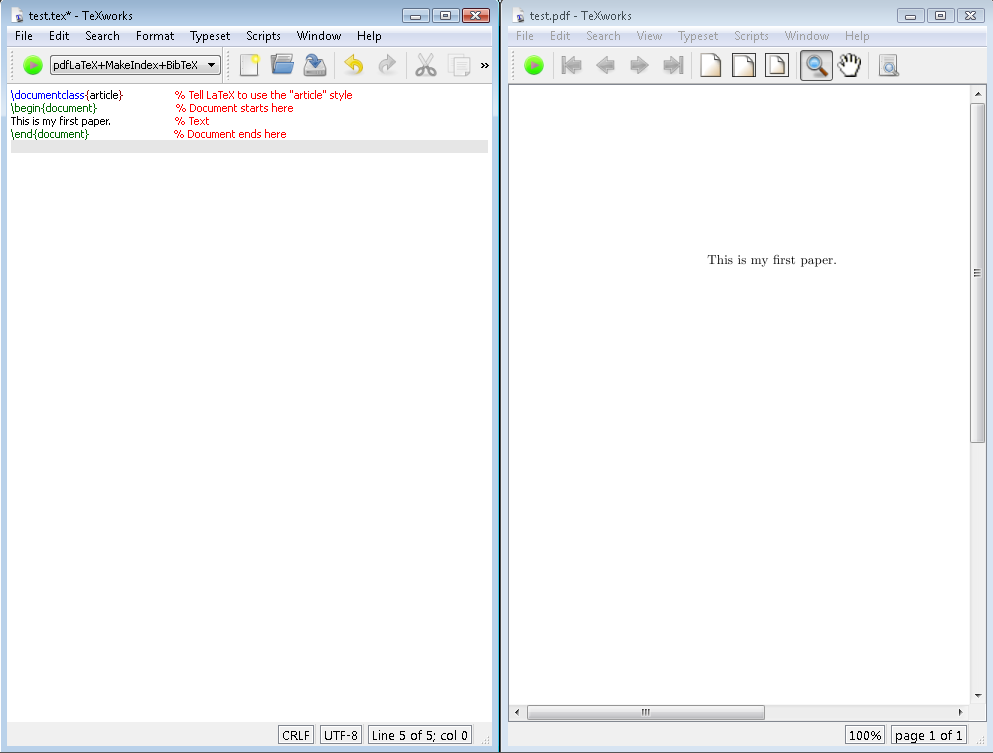
\includegraphics[width=4.75in]{figures/texworks_side}
\vspace*{.3in}
\caption{{\bf Simple document with TeXworks.} Shows syntax highlighting and simultaneous side-by-side view of text and PDF files}
\label{fig:texworks}
\end{figure}
\end{comment}
\begin{sidewaysfigure}[htbp]
\centerline{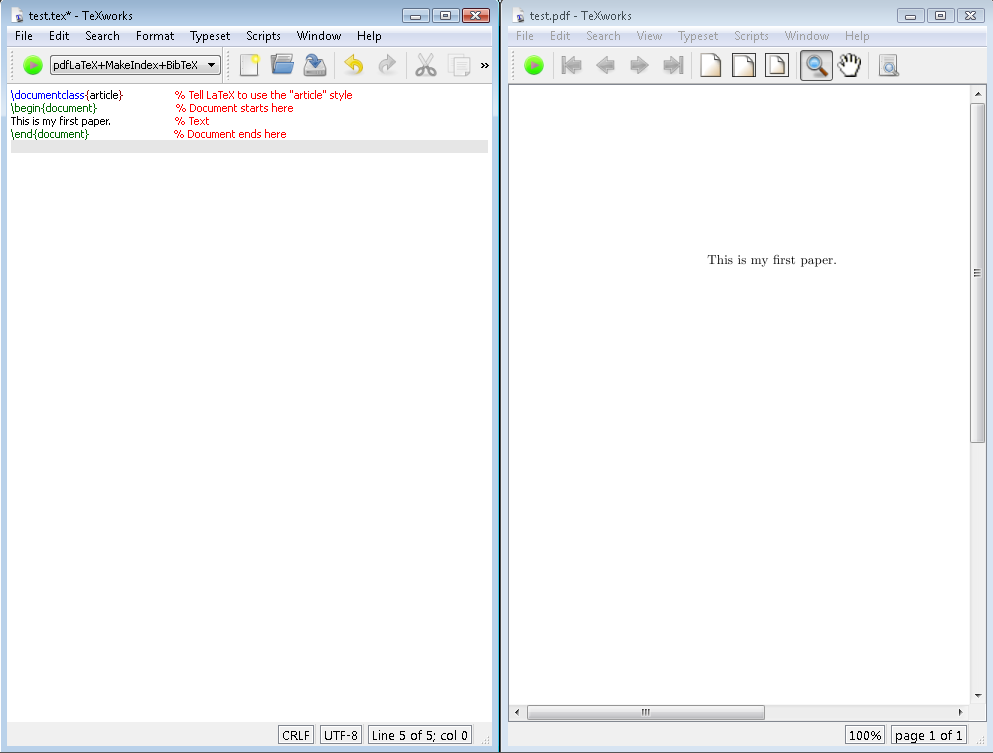
\includegraphics[height=5.5in]{figures/texworks_side}}
\vspace*{.3in}
\caption{{\bf Simple document with TeXworks.} Shows syntax highlighting and simultaneous side-by-side view of text and PDF files \rhsfn[inline,nolist]{To insert graphics, use the \texttt{\textbackslash includegraphics} command (see \texttt{graphicx} package, Section~\ref{sec:graphicx}). To create a landscape figure, use the \texttt{sidewaysfigure} environment (see \texttt{rotating} package, Section~\ref{sec:rotating}).}}
\label{fig:texworks}
\end{sidewaysfigure}
\begin{sidewaysfigure}[htbp]
\centering
%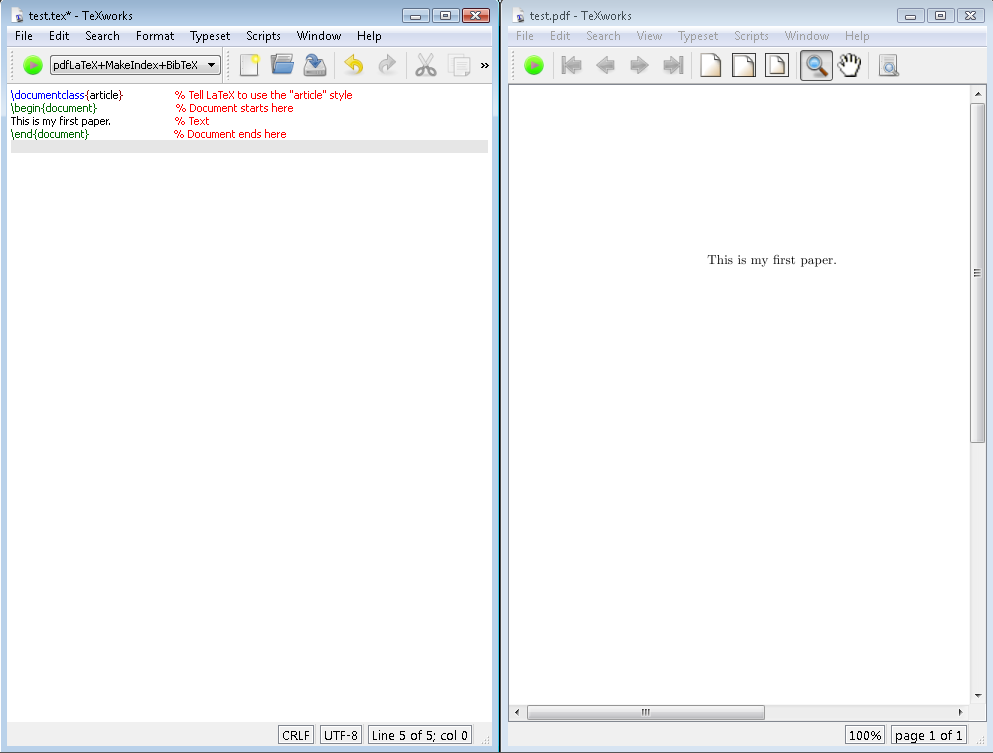
\includegraphics[height=5.5in]{figures/texworks_side}
\missingfigure[figwidth=8in]{Figure showing TeXShop}
\vspace*{.3in}
\caption{{\bf Simple document with TeXShop.} Shows syntax highlighting and simultaneous side-by-side view of text and PDF files}
\label{fig:texshop}
\end{sidewaysfigure}

\section{Introduction to \LaTeX}
\subsection{Entering text} 
Entering text is pretty straightforward---just type it. A couple of things to note if you're used to a word processor (i.e., if you are between 3 and 90 years old): i.\ \LaTeX\ doesn't care if you use one or several spaces or how often you insert a line break, and ii.\ a completely blank line tells \LaTeX\ to start a new paragraph.
\begin{example}
Lots of         spaces and
some line breaks,  but \LaTeX\
doesn't care.

A blank line tells \LaTeX\ to
start a new paragraph.
\end{example}

\noindent Start a new section or subsection using the commands \verb|\section| and \verb|\subsection|. E.g.,

% Save current section/subsection
\newcounter{sectemp}
\newcounter{subsectemp}
\setcounter{sectemp}{\value{section}}
\setcounter{subsectemp}{\value{subsection}}

% Reset (sub)section to 0 for this example
\setcounter{section}{0}
\setcounter{subsection}{0}

\settocdepth{none}             % Don't want this to show up in documents TOC.
\begin{example}
\section{Section Title}
\subsection{Subsection title}
Some very uninteresting text\ldots
\end{example}
\resettocdepth

% Reset section/subsection to original values
\setcounter{section}{\value{sectemp}}
\setcounter{subsection}{\value{subsectemp}}

\subsection{Mathematical expressions} \LaTeX\ excels at typesetting mathematical expressions. There are two ways to display them:
\begin{enumerate}[leftmargin=*]
\item {\bf Inline:} The expression appears as part of the paragraph if surrounded by (single) dollar signs, \verb|$| \ldots \verb|$|, or (equivalently) \verb|\(| \ldots  \verb|\)|. For example,
\begin{example}
Of course, $e^{i\pi} + 1 = $  
\( \lim_{x \rightarrow 0} 
\frac{\sin(x)}{x} - 1 = 0 \).
\end{example}
\item {\bf Display:} The expression appears on a separate line, with more generous vertical spacing, if surrounded by \verb|$$| \ldots \verb|$$| or (equivalently) \verb|\[| \ldots  \verb|\]|. For example,
\begin{example}
Here is a displayed equation: 
$$ E = \frac{mv^2}{2}. $$
\end{example}
\begin{example}
Here is another: 
\[ \left[\int_0^\frac{\pi}{2} 
\frac{\cos(x)}{2} \, dx\right]^3 = 
\frac{1}{8}. \]
\end{example}
\noindent There are also several environments that create \emph{numbered} equations. For example,
\begin{example}
A numbered equation:
\begin{equation}
  E = mc^2.
  \label{eq:Einstein}
\end{equation}
\end{example}
\begin{example}
Aligned, numbered equations:
\begin{align}
  \sum_{i=1}^n i &= 
    \frac{n(n+1)}{2}; \\
  \sum_{i=1}^n i^2 &= 
    \frac{n(n+1)(2n+1)}{6}.
\end{align}
\end{example}
\noindent To refer to equations in the text, use either \verb|\ref| or \verb|\eqref|:\footnote{The \texttt{\textbackslash eqref} command and \texttt{align} environment require the \texttt{amsmath} package (see Section~\ref{sec:AMS}).}
\begin{example}
Eq.~\eqref{eq:Einstein} \ldots \\
Eq.~(\ref{eq:Einstein}) \ldots
\end{example}
\end{enumerate}



\section{Useful \LaTeX\ Packages}

The standard \LaTeX\ distribution comes with a large number of extra ``packages.''  These are files with the extension .sty, which allow you to customize the behavior of \LaTeX, either by adding additional functionality or by changing the behavior of functions already defined. Many of these packages are extremely useful. For example, if you want to include graphics in your paper, you load the \texttt{graphicx} package (defined in the file \texttt{graphicx.sty}).

To use a package installed on your system, you use the command \verb|\usepackage|. For example, to load the  \texttt{graphicx} package, you'd include the command
\begin{verbatim}
\usepackage{graphicx}
\end{verbatim}
in the preamble to your document. Near the top of this file you'll find the lines
\begin{verbatim}
\usepackage{setspace,graphicx,epstopdf,amsmath,versionPO}
\usepackage{marginnote,datetime,url,enumitem,subfigure,rotating}
\end{verbatim}
These lines load some packages that I find particularly useful, and  include in almost every document I write. You can find full documentation on the Web, but here's a brief description of why each of these packages is so useful, with some brief examples illustrating their use. Before that, however, a discussion of how to install them so \LaTeX\ knows where to find them.

\subsection{Installing packages}

It's easy to use a package once it's installed on your system, but what do you have to do to install a package you haven't used before? The usual answer is ``nothing.'' Nearly all of the packages you'll ever want (including nearly all the packages described in this document) are installed as part of the \LaTeX\ distribution.\footnote{In some cases (e.g., MikTeX) you can choose not to install all packages, but to have the package manager install new packages for you whenever you ask to use them for the first time.}

\subsubsection{Installing Non-Standard Packages}
\label{sec:nonstandard}

From time to time, you may want to use a package that is not part of the standard \LaTeX\ distribution. One of the packages I use on a regular basis, \texttt{versionPO}, falls into this category, and so do my customized journal-specific files,  \texttt{jf.sty}, \texttt{jfe.sty}, and \texttt{rfs.sty}. One way to use packages like this is just to copy them into the directory containing your project's .tex file, and they will automatically be found when you process it. However, this is not a great solution, as you have to do it for \emph{every} new project, and if you ever need to edit one of these files, it's very easy to lose track of the most recent version when you have dozens of copies at various places on your disk.

A much better method is to install these files (once) somewhere \LaTeX\ will always know where to find them. This does require a bit of work, but it only has to be done once. Let's illustrate this with the \texttt{versionPO} package included with this document.

\begin{enumerate}
\item The first thing you need to decide is where to put your extra .sty file(s). You could put them in the same directory structure as the standard packages, but  don't do this.\footnote{When you next upgrade your installation, you'll have to remember to copy them elsewhere (which also means remembering which packages they were) to avoid losing them.} Instead, set up your own local directory tree. For example, on my Windows system, I store extra packages in subdirectories under \verb|c:\RHS\texmf-local\tex\latex|, and on my Mac I use
\verb|/Users/stanton/Library/texmf/tex/latex|.\footnote{This may seem complicated, but it follows the recommended \TeX\ directory structure. \ifcomment{Similarly, my extra font files are installed in \texttt{c:\textbackslash RHS\textbackslash texmf-local\textbackslash fonts} and bibliography-related files in \texttt{c:\textbackslash RHS\textbackslash texmf-local\textbackslash bibtex} (see Section~\ref{sec:bib}).}{} You can pick anywhere you like for the root of this directory structure (\texttt{c:\textbackslash RHS\textbackslash texmf-local}, for example), but everything underneath this directory should follow the standard structure. For additional information on the standard \TeX\ directory structure (TDS), see \url{http://www.tex.ac.uk/tex-archive/tds/tds.html}).}
\item After creating the relevant directory, tell your \LaTeX\ installation where to find it. 
  \begin{itemize}
  \item MikTeX 2.09:
    \begin{itemize}
    \item  From the Windows program menu, select MikTeX 2.09 $\rightarrow$ Maintenance (Admin) $\rightarrow$ Settings (Admin).
    \item Click on the ``Roots'' tab, click ``Add,'' and select the appropriate directory structure (in my case, 
      this is \verb|c:\RHS\texmf-local|).\footnote{This will allow \LaTeX\ to find files anywhere under this directory.}
    \end{itemize}
  \item TeX Live (MacTeX):
    \begin{itemize}
      \item If you chose the same directory as I did (\verb|~/Library/texmf/tex/latex|, where \verb|~| denotes your own home directory, e.g., \verb|/Users/stanton|), \LaTeX\ will automatically look for files there and in all subdirectories, so you don't need to do anything else here.

\begin{comment}
    \item Use any text editor to open the file \texttt{/usr/local/texlive/2011/texmf.cnf}.\footnote{This assumes your version of MacTeX is based on TeX Live 2011. If it's based on TeX Live 2010, say, replace 2011 with 2010 in the directory name.}\footnote{Opening files in this directory under OS X is not that easy as OS X tries to ``protect'' you from deleting important files by not allowing you to see them in Finder (or many other applications) at all. There are various ways to see this directory, but the simplest within Finder is to select the ``Go'' menu, then ``Go to Folder'', then enter the path (in this case, \texttt{/usr/local/texlive/2011}. Finder will now show the contents of this folder, and you can make it permanently available by dragging it to the sidebar. \rhsfn{Verify this.}}
    \item Point \texttt{TEXMFHOME} to wherever you want your personal directory structure to reside. For example, on my system, \texttt{texmf.cnf} contains the line 
\begin{verbatim}
TEXMFHOME = ~/tex/texmf-local
\end{verbatim}
    \end{comment}
  \end{itemize}
\end{itemize}
\end{enumerate}
\textbf{Note:} Both of these steps only need to be done once for a given \LaTeX\ installation. The next steps need to be performed for every non-standard package you install.
\begin{enumerate}[resume]

\item Copy any new .sty files into the directory structure you just created. For example, \verb|c:\RHS\texmf-local\tex\latex\misc\versionPO.sty|.
\end{enumerate}
Now run \LaTeX\ on a file that uses the package \texttt{versionPO}. Wait! It fails with the error message \rhs[nolist]{Should work OK with the Mac; verify.}
\begin{verbatim}
! LaTeX Error: File `versionPO.sty' not found.
\end{verbatim}
What the\ldots?! \LaTeX\ knows where you want to keep your extra files and you've put the file right where \LaTeX\ expects to find it. This is a very frustrating error, which can cause people to get quite annoyed with the idiot coauthor who told them to install a non-standard package on their system (or so I've heard\ldots). The reason for the error (which is easy to forget even for experienced \LaTeX\ users, leading to potential frustration \emph{every} time you install a new non-standard package) is that when you run \LaTeX, it doesn't actually search in every relevant directory to find all the files it needs to load; this would make it unbearably slow. Instead, it consults a database that tells it where to find each file. Each time you install a new file, there's therefore one additional step:
\begin{enumerate}[resume]
\item Update the \LaTeX\ file name database.
  \begin{itemize}
  \item MikTeX 2.09:
    \begin{itemize}
    \item  From the Windows program menu, select MikTeX 2.09 $\rightarrow$ Maintenance (Admin) $\rightarrow$ Settings (Admin).
    \item Click on ``Refresh FNDB'' (\textbf{F}ile \textbf{n}ame \textbf{d}ata\textbf{b}ase).
    \end{itemize}
  \item TeXLive (MacTeX):
    \begin{itemize}
    \item Run the command \texttt{texhash} or \texttt{mktexlsr}. \rhs[nolist]{Shouldn't need to do this if we chose the default location.}
    \end{itemize}
  \end{itemize}
\end{enumerate}

\subsection{Changing line spacing: \texttt{setspace}}

Journals often want submissions to be double-spaced, while for most purposes I use 1.5 spacing. \texttt{setspace} is a convenient way to set or change the line spacing of the document, or parts of the document. For example, near the top of this file is the command
\begin{verbatim}
\onehalfspacing
\end{verbatim}
This sets the overall document spacing to one and a half. You can also single-space part of the text (the abstract, say) by enclosing it in a \texttt{singlespace} environment:

\begin{example}
\begin{singlespace}
This is single spaced. Once this 
environment is finished, the document 
will revert to its previous spacing.
\end{singlespace}
\end{example}

\subsection{Including figures: \texttt{graphicx}}
\label{sec:graphicx}

Use this package to include figures in your document. For example, here's a picture of the MikTeX settings page described in footnote~\ref{fn:miktex} on page~\pageref{fn:miktex}.

\begin{example}
\begin{figure}[H]
\centering
\includegraphics%
[width=1in]{figures/MikTeX_Options}
\caption{MikTeX main options page}
\label{fig:MikOptions}
\end{figure}
\end{example}

\noindent \textbf{Notes} 
\begin{itemize}
\item Don't include the extension in the file name. The package knows about several standard graphics types (in this example, I provided a PNG file). In particular, if you tell it to look for 
``file'' then if you process the file straight to PDF using pdf\LaTeX{}, it will automatically look for ``file.pdf'' (\texttt{pdflatex} can't handle EPS files) and if you're processing it to a DVI file (and then to a PS file) using the ``latex'' command, it will automatically look for ``file.eps'' (\texttt{latex} can't handle PDF files). 
\item If the \texttt{pdflatex} command cannot handle EPS files, what do you do if you don't want to convert your source file to .dvi, but only have EPS graphic files?\footnote{For example, Matlab is much better at generating EPS files than PDF files.} The answer is to include the \texttt{epstopdf} package, which automatically converts all EPS graphics files to PDF files on the fly when you process the source using \texttt{pdflatex}.
\item There are various options for telling \LaTeX{} where to put a figure on the page. In this case I wanted to force \LaTeX\ to put the figure exactly where I defined it, so I used the \texttt{[H]}  option, defined in the \texttt{float} package.
\end{itemize}


\subsection{Mathematical typesetting: \texttt{amsmath}}
\label{sec:AMS}
Contains lots of useful extra mathematical features, fonts, etc. Some of the most useful:
\subsubsection{\textbackslash eqref}
This puts parentheses around equation numbers for you instead of your doing it manually with \texttt{\textbackslash ref}. For example,\footnote{Yes, I realize both versions have the same number of characters, but for my two-fingered typing style it's quicker to type an extra ``eq'' than the two parentheses.}
\begin{example}
Equation~(\ref{eq:Emc2}) versus \\
Equation~\eqref{eq:Emc2}.
\end{example}

\subsubsection{\textbackslash begin\{align\} \ldots \textbackslash end\{align\}} 
Use this instead of \texttt{eqnarray} for aligning multiple equations. 
Compare the spacing of the following equations:
\begin{example}
\begin{equation}
E = mc^2. 
\end{equation}
\end{example}
\begin{example}
\begin{align}
E &= mc^2. \\
A &= \pi r^2.
\end{align}
\end{example}
\begin{example}
\begin{eqnarray}
E &=& mc^2. \\
A &=& \pi r^2.
\end{eqnarray}
\end{example}
\noindent \textbf{Note:} \cite{OetikerPartlHynaSchlegl:11} recommend using \texttt{IEEEeqnarray} (part of the \texttt{IEEEtrantools} package) instead of \texttt{align} \citep[see][for details on this environment and lots of useful discussion of how to typeset mathematical equations]{Moser:12}. It does seem to overcome some drawbacks of the \texttt{align} package, and maybe I'll try it out one day\ldots. For now, here's the same example as above:\footnote{One negative: \texttt{IEEEtrantools} is not part of the MiKTeX distribution, so you'll have to install it manually. All of my coauthors already hate me for making them learn how to install non-standard packages\ldots (see Section~\ref{sec:nonstandard}). In addition, \texttt{IEEEtrantools} interacts badly with \texttt{enumitem} unless you load it with the command \texttt{\textbackslash usepackage[retainorgcmds]\{IEEEtrantools\}}.}

\begin{example}
\begin{IEEEeqnarray}{rCl}
E &=& mc^2. \label{eq:Emc2} \\
A &=& \pi r^2.
\end{IEEEeqnarray}
\end{example}

\subsubsection{\textbackslash begin\{cases\} \ldots \textbackslash end\{cases\}} 
Useful when an equation's right-hand side can take several forms. For example,
\begin{example}
\begin{equation}
C(S) =  \begin{cases}
0 & \text{if $S \leq K$}, \\
S - K & \text{otherwise}.
\end{cases}
\end{equation}
\end{example}

\subsection{Setting page margins: \texttt{geometry}}

A convenient way to set the page layout, margins, etc.\footnote{For some reason, the default \LaTeX\ margins are huge.} For example, to set one-inch margins on all sides, you simply type
\begin{verbatim}
\usepackage[margin=1in]{geometry}
\end{verbatim}
This can all be done manually instead, but it takes a lot more work.

\subsection{Inserting notes: \texttt{todonotes}}
\label{sec:todo}

An extremely useful package for adding notes.\footnote{For full details, see the package documentation at \url{http://www.ctan.org/tex-archive/macros/latex/contrib/todonotes/todonotes.pdf}.} \label{firstnote}\rhs[caption={\textbf{RS:} Dear author, this is gibberish.}]{(Sample note) Dear author, this is gibberish. Note that this note appears both here and in the global To Do list on page~\pageref{sec:listoftodos}. Note also that I used the \texttt{caption} to create a shorter entry for the To Do list.} These can either be in the text or in the margin, can be colored as you desire, can appear in a global To Do list or not, can easily be switched off whenever you need to print a neat version of the paper, etc. I usually use marginal notes, and set the margins and paper size so that the layout doesn't change (much) when you turn notes on or off (see also Section~\ref{sec:version}).\footnote{You also need to include the \texttt{marginnote} package if you want to generate notes in footnotes.}
This package has lots of different options. I define my default note command, \verb|\rhs|, as follows: %\rhs{Examples using \texttt{\textbackslash todo} command.}
\begin{verbatim}
\newcommand{\smalltodo}[2][] {\todo[caption={#2}, size=\scriptsize,%
 fancyline, #1]{\begin{spacing}{.5}#2\end{spacing}}}
\newcommand{\rhs}[2][]{\smalltodo[color=green!30,#1]{{\bf RS:} #2}}
\end{verbatim}
The command \verb|\rhs| produces (by default) a green margin note with a small font and tight interline spacing (to allow me to get more text into a cramped space), and inserts a nice arrow pointing to the relevant point in the text.\footnote{You need to run 
\LaTeX\ several times to get the note and arrow correctly placed.} \rhsnolist{Like this one, inserted with the command \texttt{\textbackslash rhs\{Like this one, inserted with the command \textbackslash rhs\{Like this one, inserted\ldots}}
The note is also listed by default in the global To Do list, if there is one. This list, which summarizes the notes in the entire paper, can be inserted anywhere in your text (usually at the top) with the command \verb|\listoftodos|:
\begin{example}
\listoftodos[Richard's To Do List]
\end{example}
\label{sec:listoftodos}
\noindent This is useful for keeping track of large numbers of notes, but I often don't include it as it changes the layout of the paper (and the notes are pretty easy to see in the text anyway).
\noindent You can easily modify the definition of or add additional options to the \verb|\rhs| command to create different results. For example, it's easy to change the color \rhs[color=red!30,caption={{\bf RS:} A red note}]{A red note, inserted with the command 
\texttt{\textbackslash rhs[color=red!30]\{A red note, inserted with the command \ldots}} or to make an inline note.
\begin{verbatim}
\rhs[inline,nolist]{Here's an inline note. I don't use these much as 
the paper's spacing changes when you turn them off, but they're useful 
if you have a really long note. This note does not appear in the To Do 
list because I used the \texttt{nolist} option.}
\end{verbatim}
\rhs[inline,nolist]{Here's an inline note. I don't use these much as the paper's spacing changes when you turn them off, but they're better if you have a really long note. This note does not appear in the To Do list because I used
the \texttt{nolist} option.}

\paragraph{Note:} By default, todo notes do not work inside footnotes or floats (figures and tables). If you try, \LaTeX\ produces an incomprehensible error message and no note. A work-around for this problem is to redefine the command \verb|\marginpar| using the command\footnote{This requires you to load the \texttt{marginnote} package.}
\begin{verbatim}
\renewcommand{\marginpar}{\marginnote}
\end{verbatim}
This allows notes to be created inside footnotes, but you will now find that notes on your page overlap if you create two notes close together in the text. To prevent this, my current work-around is \emph{not} to include the command above, but instead to define a new note command \verb|\rhsnfn|, to be used only in footnotes and floats, which performs this redefinition temporarily. This is done by the following lines at the top of this document:
\begin{verbatim}
\let\oldmarginpar\marginpar   % Save original definition of \marginpar
\newcommand{\rhsfn}[2][]{%  To be used in footnotes and floats
\renewcommand{\marginpar}{\marginnote}%
\smalltodo[color=green!30,#1]{{\bf RS:} #2}%
\renewcommand{\marginpar}{\oldmarginpar}}
\end{verbatim}


\subsection{Printing date and time: \texttt{datetime}}
\label{sec:datetime}

Allows various choices of formatting dates, as well as referring to the current time (via \verb|\currenttime|). This is useful for mammoth editing sessions where you've created printouts of several different versions of a document during the same day.

\subsection{Multiple versions from one file: \texttt{versionPO}}
\label{sec:version}

This package allows you to include text in your paper conditionally, so you can generate multiple different versions of a document from a single source file by changing just one or two statements.\footnote{One drawback of \texttt{versionPO.sty} is that it's not included as part of the standard \LaTeX\ installation. I've therefore included it with this document, and it needs to be installed as described in Section~\ref{sec:nonstandard}. \texttt{versionPO.sty} was written by Piet van Oostrum in about 1991 and originally named version.sty. I renamed it versionPO.sty to avoid any possible conflicts with a different file, also called version.sty, that \emph{is} in the standard distribution.There are several standard packages that do similar things to this one, including \texttt{version}, \texttt{versions}, \texttt{optional}, and \texttt{comment}. You should feel free to use one of them instead, but I am used to using \texttt{versionPO} and don't like change.} 
here are many, \emph{many} uses for this package, including 
\begin{itemize}
\item Creating working papers and journal submissions from a single source file.
\item Optionally including responses to referees.
\item Adding notes to yourself that you can switch on or off at will.
\item Writing an exam and having the option to add extra space for students to write their answers, or having the option to include solutions, again all in a single file.
\end{itemize}
Here's a simple example. See what happens to the output below when you change the command \verb|\includeversion{notes}| to \verb|\excludeversion{notes}| at the top of the file.

\begin{example}
Notes \ifnotes{\emph{are}}%
{are \emph{not}} shown in this file.
\end{example}
\noindent A slightly more interesting example is the following, from the top of this file:
\begin{verbatim}
\ifnotes{%
\usepackage[margin=1in,paperwidth=10in,right=2.5in]{geometry}%
\usepackage[textwidth=1.4in,shadow,colorinlistoftodos]{todonotes}%
}{%
\usepackage[margin=1in]{geometry}%
\usepackage[disable]{todonotes}%
}
\end{verbatim}
If the command \verb|\includeversion{notes}| appears at the top of this file, then this command loads \texttt{todonotes} with various options, and then loads \texttt{geometry} with some slightly strange paper size and margin definitions that allow both the text and the margin notes to be printed on a standard piece of paper without changing the text layout. \rhs[nolist]{To maximize how much I can say, I use a small font and the widest margin notes I can get my printer to generate.} If  the command \verb|\excludeversion{notes}| appears instead, notes are disabled and standard one-inch margins are used, producing a version of the document ready for distribution. One environment defined by default (and excluded) is \texttt{comment}, so you can comment out text by either surrounding it with \verb|\ifcomment{...}| or (useful for larger blocks) putting it inside \verb|\begin{comment}|  \ldots \verb|\end{comment}|. This is useful for temporarily removing text that you might want to put back later. For example,
\begin{example}
This is the first sentence.
\begin{comment}
The second sentence is commented out.
\end{comment}  
This is the third sentence.
\end{example}
\noindent Here are some more examples from the top of this document. Try changing their settings to see what happens when you reprocess the document.
\begin{verbatim}
\includeversion{notes}          % Include notes?
\includeversion{links}          % Turn hyperlinks on?
\excludeversion{submit}         % Format for conference submission?
\includeversion{toc}            % Include table of contents?
\end{verbatim}

\subsection{List formatting: \texttt{enumitem}}
\label{sec:enumitem}

\texttt{enumitem} enables easy control over many aspects of numbering and spacing in enumerate, itemize, and description lists. For example, at the top of this file you'll see the command
\begin{verbatim}
\setlist{noitemsep}
\end{verbatim}
This removes all extra vertical space between list items, which I prefer to the default spacing (by default, \LaTeX\ puts extra 
vertical space between list items). You can also use this package to change the indentation of a list. For example, 
\begin{example}
Here is an unindented itemized list:
\begin{itemize}[leftmargin=*]
\item Item 1.
\item Item 2.
\end{itemize}
\end{example}

\subsection{URLs and hyperlinks: \texttt{hyperref}}
\label{sec:hyperref}

This package allows you to include clickable hyperlinks in your paper for URLs, citations, equations, references, etc. For example,
\begin{example}
\cite{Stanton:95} \\
\url{http://www.ctan.org/} \\
\href{http://www.ctan.org/}%
  {CTAN Web site} \\
Equation~\eqref{eq:Emc2} \\
Section~\ref{sec:todo}
\end{example}
\noindent You can customize how (and if) these are displayed in your text (colored text, boxes, etc.). There are also unlinked versions of some commands, e.g.,
\begin{example}
\nolinkurl{http://www.ctan.org/}
\end{example}
\noindent If you don't want any hyperlinks in your document, you can 
turn them all off with the command \verb|\hypersetup{draft=true}|.\footnote{An alternative is to use the \texttt{url} package, but it is less flexible than \texttt{hyperref}.} You can try this out by changing the command \verb|\includeversion{links}| to \verb|\excludeversion{links}| at the top of this document.

\subsection{Landscape and subfigures: \texttt{rotating} and \texttt{subfigure}}
\label{sec:rotating}

The \texttt{rotating} package allows the creation of tables and figures in landscape mode using 
\verb|\begin{sidewaystable}|  \ldots \verb|\end{sidewaystable}| for tables and
\verb|\begin{sidewaysfigure}|  \ldots \verb|\end{sidewaysfigure}| for figures.\footnote{Note that these are placed on separate pages. This is usually what you want, as you're rotating the figure or table because it's too large to be set in portrait mode. However, there is also the \texttt{sideways} environment, which allows you to have rotated text/figures on the same page as non-rotated material.}
The \texttt{subfigure} package allows creation of a single figure with multiple subfigures. Figure~\ref{fig:fig_subfig}  illustrates the use of both \texttt{rotating} and \texttt{subfigure}, created using the command
\begin{verbatim}
\begin{sidewaysfigure}
\begin{center}
\subfigure[A somewhat familiar figure]{
  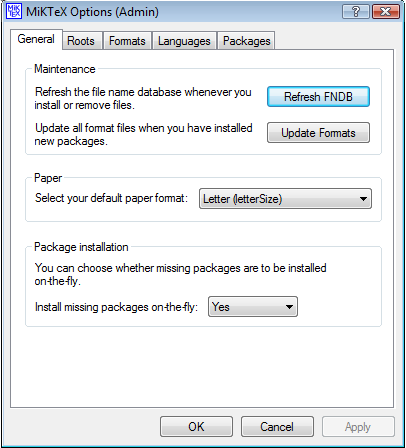
\includegraphics[width=3.5in]{figures/MikTeX_Options}
  \label{fig:sub1}
}
\subfigure[That was fun. Let's plot it again!]{
  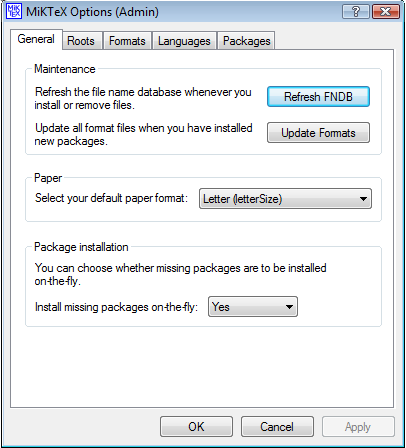
\includegraphics[width=3.5in]{figures/MikTeX_Options}
  \label{fig:sub2}
}
\end{center}
\caption{This completely gratuitous figure plots the same graphic 
we saw earlier, but does so twice and in landscape mode. How exciting!
}
\label{fig:fig_subfig}
\end{sidewaysfigure}
\end{verbatim}
Note that you can also refer to the whole figure or to individual subfigures in the text, e.g., 
\begin{example}
  Figure~\ref{fig:fig_subfig}. \\
  Figure~\ref{fig:sub2}.
\end{example}
\begin{sidewaysfigure}
\begin{center}
\subfigure[A somewhat familiar figure]{
  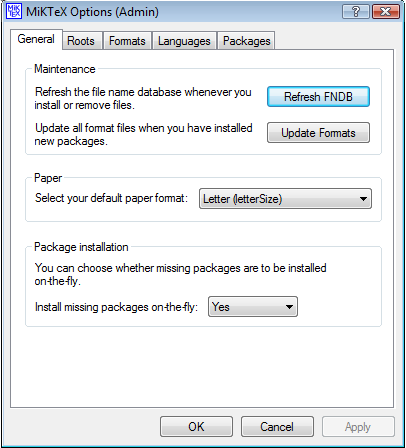
\includegraphics[width=3.5in]{figures/MikTeX_Options}
  \label{fig:sub1}
}
\subfigure[That was fun. Let's plot it again!]{
  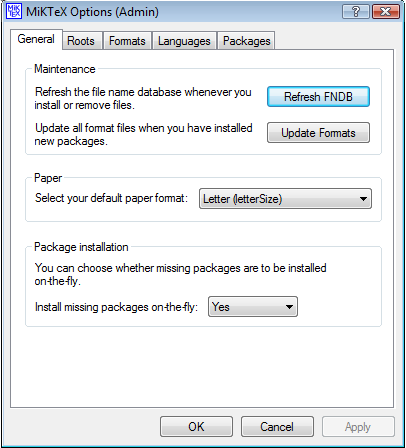
\includegraphics[width=3.5in]{figures/MikTeX_Options}
  \label{fig:sub2}
}
\end{center}
\caption{This completely gratuitous figure plots the same graphic we saw earlier, but does so twice and in landscape mode. How exciting!
}
\label{fig:fig_subfig}
\end{sidewaysfigure}

\subsection{Other useful packages}

Though I don't use these in every document, here are a few other packages I sometimes find useful:
\begin{itemize}
\item \texttt{bibunits:}  Allows you to create multiple bibliographies in a single document. For example, you might be teaching a class and want a single document with a section on each of a number of topics and a separate bibliography per section. You can optionally also have a single global bibliography. Each bibliography can have a different format.
\item \texttt{tocvsec2:} Allows you to control which level of section appears in the table of contents, and you can change this section by section. For example, you might want to list subsections from the main body of the paper, but only sections from the Appendix.
\item \texttt{lastpage:} Allows you to refer to the number of the last page of the document.
\item \texttt{tikz:} Very powerful environment for creating diagrams.
\item \texttt{indentfirst:} Indents the first line of a new section (JF asks for this).
\item \texttt{caption:} Gives you easy control over the format of figure and table captions. Useful for satisfying journal requirements.
\item \texttt{xr:} Allows you to refer in one document to labels in another document. Useful, for example, for creating an Internet Appendix for the Journal of Finance where you want to be able to refer to equation numbers in the main paper.\footnote{This could alternatively be done by putting everything in a single file and using \texttt{bibunits} to generate the two (separate) bibliographies, but then you'd need to split the resulting PDF file in half. It's your choice.}
\item \texttt{amsthm:} Allows good control over theorem-like environments.
\item \texttt{booktabs:} Allows good control over table layout and spacing.
\item \texttt{longtable:} Allows a single table to span more than one page, keeping the same column headings, etc.
\end{itemize}

\section{Citations and Bibliographies}
\label{sec:bib}

\LaTeX{} makes it very easy to create and format citations and bibliographies. The most basic method is to insert the bibliography manually into your paper using the \texttt{thebibliography} environment and one \verb|\bibitem| command for each entry. E.g.,
\begin{verbatim}
\begin{thebibliography}{99}
\bibitem{Stanton:95} Stanton, Richard, 1995, Rational prepayment and the 
value of mortgage-backed securities, {\em Review of Financial Studies\/} 
8, 677--708.
\end{thebibliography}
\end{verbatim}
This entry would be cited in the text using the command \verb|\cite{Stanton:95}|. 

This is how bibliography creation is described in \cite{Lamport:94} and \cite{OetikerPartlHynaSchlegl:11} (though the latter does mention using Bib\TeX), but \texttt{don't do it this way!} Major drawbacks of this manual method include:
\begin{enumerate}
\item If you remove a citation from your text, you need to remove that paper from the bibliography manually (after, of course, checking to make sure you're not still citing it somewhere else).
\item To match a journal's bibliography style, you have to edit every entry by hand.
\item Since there's no central database of references, you typically end up having to retype (after re-Googling) the same citations over and over again in different papers. This is both time-consuming and error-prone.
\item By default, \LaTeX{} produces numerical citations, whereas most finance journals want author-year citations, e.g.,  \cite{Stanton:95}.
\end{enumerate}

\subsection{Bib\TeX{}}

The solution to the problems above is to create bibliographies using Bib\TeX, a separate program installed as part of any standard \LaTeX{} installation.\footnote{One day, it will probably be even better to use the \texttt{biblatex} package instead. This has some more features than Bib\TeX\ (for example, you can have citations appear in footnotes, and can refer to the title of a reference within your text), and it is in principle easier to customize, but it is \emph{currently} easier to generate journal-specific bibliography formats using Bib\TeX\ with \texttt{custom-bib}.} Compared with the manual method,
\begin{enumerate}
\item Bib\TeX\ automatically inserts only references you actually cite (or that you tell it to insert even though you don't actually cite them, using the \verb|\nocite| command). If you delete all citations to a particular paper, it will automatically be removed from your bibliography.
\item Reformatting a bibliography usually requires editing just a single command in your paper (see Section~\ref{sec:custom-bib}).
\item You keep all references in a central database. As a result,
  \begin{enumerate}
  \item You only need to type or look each reference up once.
  \item There's no doubt about where to find the latest version of any reference.
  \item Once you've corrected any errors in a reference, they remain corrected forever.
  \end{enumerate}
\item It's easy to generate citations in any format you desire, especially author-year format, using just the standard \verb|\cite| command (see Section~\ref{sec:natbib}).
\end{enumerate}

\subsection{The Bib\TeX\ database}

When using Bib\TeX, you store all your references in one or more .bib files, taking the following format:
\begin{verbatim}
@ARTICLE{Stanton:95,
  author = {Richard Stanton},
  title = {Rational Prepayment and the Value of Mortgage-Backed Securities},
  journal = {Review of Financial Studies},
  year = {1995},
  volume = {8},
  pages = {677--708},
  number = {3}
}
\end{verbatim}
Note that this entry contains all of the logical information about the reference (author, title, etc.), but says nothing about   formatting, which is handled separately. Once you've entered a reference in your .bib file and told \LaTeX\ and Bib\TeX\ where to find it (see below), when you use the \verb|\cite| command, Bib\TeX{} will automatically find the right reference, add it to your bibliography, and insert the appropriate citation in the text, e.g.,
\begin{example}
\cite{Stanton:95}
\end{example}
Just like a .tex file, a .bib file is a plain-text file and can be edited with the same editor you use to edit your .tex files. However, there are also some Bib\TeX-specific editors, including JabRef (available on multiple platforms from 
\url{http://jabref.sourceforge.net}) and BibDesk (OS X only, installed as part of the MacTeX distribution).

\subsection{Telling Bib\TeX\ where to find the database}

You tell Bib\TeX{} to look for references in the file \texttt{master.bib} by putting the following line in your TeX file:
\begin{verbatim}
\bibliography{master}
\end{verbatim}
\textbf{Note:} Bib\TeX{} will always find the file master.bib if it is in the current directory, but you don't want to have lots of different versions of this file sitting in every different project directory. A better approach is to set the environment variable \texttt{BIBINPUTS} to point to the directory in which you've stored your Bib file, and then Bib\TeX{} will find it no matter where you run it from. 
\begin{itemize}
\item On my Windows machine, \texttt{BIBINPUTS} is set to \texttt{c:/RHS/texmf-local/bibtex/bib//}, which will look for Bib files in the current directory and then, failing that, in directory \verb|c:\RHS\texmf-local\bibtex\bib| and in all subdirectories.\footnote{Searches in Windows almost always look in the current directory first, so this doesn't need specifying.}
\begin{itemize}
\item To set an environment variable in Windows, go to Control Panel and select System $\rightarrow$ Advanced $\rightarrow$ Environment Variables. Then under ``System Variables,'' click ``New,'' enter the variable name (\texttt{BIBINPUTS}) and the variable value (\texttt{c:/RHS/texmf-local/bibtex/bib//}, and click OK a few times.
\end{itemize}
\item On my Mac, \texttt{BIBINPUTS} is set to \texttt{./:/Users/stanton/tex/texmf-local/bibtex/bib//},
which will look for Bib files in the current directory and, failing that, in the directory \verb|c:\RHS\texmf-local\bibtex\bib| and in all its subdirectories.
\begin{itemize}
\item To set an environment variable in OS X, edit file \verb|~/.profile| and add the line\footnote{Strictly speaking, this only has an effect if you're running \LaTeX\ from a command shell. If run from within a GUI application, this may not work. If this is a problem for you, set the environment variable instead using the command \texttt{launchctl setenv BIBINPUTS \nolinkurl{./:~/tex/texmf-local/bibtex/bib//}.}}
\begin{verbatim}
export BIBINPUTS=./:~/tex/texmf-local/bibtex/bib//
\end{verbatim}
\end{itemize}
\end{itemize}

\subsection{Formatting the bibliography: \texttt{natbib} and  \texttt{custom-bib}}

\subsubsection{natbib}
\label{sec:natbib}

This package provides finer control than basic \LaTeX{} over citation formatting. For example,
\begin{example}
\cite{Stanton:95} \\
\citep[see, for example,]%
       [p. 3]{Stanton:95} \\
\citet[Equation~1]{Stanton:95} \\
\citealt[Equation~1]{Stanton:95} \\
\citealp[Equation~1]{Stanton:95} \\
\citeauthor{Stanton:95} \\
\citeyear{Stanton:95}
\end{example}
\noindent By loading the extra package \texttt{bibentry}, you can also print the full reference. For example,
\begin{example}
\bibentry{Stanton:95}
\end{example}

\subsubsection{Customizing the bibliography format: custom-bib}
\label{sec:custom-bib}

This package allows you to define a new bibliography style ( a .bst file), matching the format of your bibliography to that of the journal you are submitting to.\footnote{You can alternatively create or edit the appropriate .bst file by hand. However, before you even think of doing this, take a look at one of the .bst files in your \LaTeX{} installation. These use a mysterious syntax that is most definitely \emph{not} fun to edit\ldots}
To create a new bibliography style called, say, \texttt{jf.bst} for the \emph{Journal of Finance}, run the command
\begin{verbatim}
latex makebst
\end{verbatim}
and then answer various questions about the name of the output file and how you want your bibliography formatted. It then creates a customized .bst file, jf.bst. To use the format defined in this file, you insert the command
\begin{verbatim}
\bibliographystyle{jf}
\end{verbatim}
in your document. This tells \LaTeX{}/Bib\TeX{} to format the bibliography using information in the file jf.bst. 

\section{Journal-Specific Document Formatting}

Journals typically have their own requirements for section numbers,
figure captions, etc., as well as for the format of the
bibliography. Meeting these requirements requires you to modify some
of the default definitions.

\subsection{Formatting the bibliography}
\label{sec:bibjournal}

I've used \texttt{custom-bib} to create bibliography styles for 
\begin{itemize}
\item \emph{Journal of Finance} (\textbf{jf.bst}),
\item \emph{Journal of Financial Economics} (\textbf{jfe.bst}),
\item \emph{Review of Financial Studies} (\textbf{rfs.bst}).
\end{itemize}
These files are included with this document. 
Change the command \verb|\bibliographystyle{jf}| below to \verb|\bibliographystyle{jfe}| or \verb|\bibliographystyle{rfs}|, reprocess the document  (by running LaTeX, BibTeX, and LaTeX again), and see how the bibliography format changes.\footnote{The bibliography contains references to published papers \citep{Stanton:95}, books \citep{Hull:11}, and working papers \citep{CarpenterStantonWallace:12}, so you can see how various entry types are formatted.}

\textbf{Note:}  You'll typically find one or two minor journal bibliography conventions that custom-bib can't quite handle.\footnote{For example, you may have page numbers listed in your Bib\TeX{} database as ``1023--1045'', while the journal insists on ``1023--45''.} You now have two choices. One is to spend hours manually editing the .bst file to do what you want. The other (which I recommend) is to wait until the bibliography is really final, then just copy the contents of the \texttt{.bbl} file into the body of the text  (removing the \verb|\bibliographystyle| and \verb|\bibliography| commands), and  edit it manually to make these last few changes.\footnote{Save even more time by doing this \emph{after} the copy-editor has taken a look and pointed out where you need to make changes.}

\subsection{Formatting the text}
\label{sec:textjournal}

In addition to the bibliography format files mentioned above, I have also have written style files to help make your paper match the submission requirements of either the
\emph{Journal of Finance} (\texttt{jf.sty}), \emph{Journal of Financial Economics} (\texttt{jfe.sty}), or \emph{Review of Financial Studies} (\texttt{rfs.sty}).
I have also included a sample ``paper'' for each journal, which you can use as the basis for preparing your own documents. They include similar packages to this document, but each also includes the journal-specific style file and bibliography format file, and also has some journal-specific formatting commands in the text. The specific files included for each journal are:
\begin{enumerate}
\item {\bf Journal of Finance:}
  \begin{itemize}
  \item \href{../jf/jf.sty}{jf.sty}: Formatting commands for papers.
  \item \href{../jf/jfIA.sty}{jfIA.sty}: Formatting commands for Internet Appendices.
  \item \href{../jf/jf.bst}{jf.bst}: Bibliography format.
  \item \href{../jf/jfsample.tex}{jfsample.tex}: Sample paper (\TeX\ file).
    \begin{itemize}
    \item \href{../jf/jfsample.pdf}{PDF file}.
    \end{itemize}  
  \item \href{../jf/jfIAsample.tex}{jfIAsample.tex}: Sample Internet Appendix (\TeX\ file).
    \begin{itemize}
    \item \href{../jf/jfIAsample.pdf}{PDF file}.
    \end{itemize}
  \end{itemize}
\item {\bf Journal of Financial Economics:}
  \begin{itemize}
  \item \href{../jfe/jfe.sty}{jfe.sty}: Formatting commands for papers.
  \item \href{../jfe/jfe.bst}{jfe.bst}: Bibliography format.
  \item \href{../jfe/jfesample.tex}{jfesample.tex}: Sample paper (\TeX\ file).
    \begin{itemize}
    \item \href{../jfe/jfesample.pdf}{PDF file}.
    \end{itemize}  
  \end{itemize}
\item {\bf Review of Financial Studies:}
  \begin{itemize}
  \item \href{../rfs/rfs.sty}{rfs.sty}: Formatting commands for papers.
  \item \href{../rfs/rfs.bst}{rfs.bst}: Bibliography format.
  \item \href{../rfs/rfssample.tex}{rfssample.tex}: Sample paper (\TeX\ file).
    \begin{itemize}
    \item \href{../rfs/rfssample.pdf}{PDF file}.
    \end{itemize}  
  \end{itemize}
\end{enumerate}










\section{Working with Others: Version Control Systems}
\label{sec:VCS}

When working on a paper with other people, you have to be careful to keep track of who is working on what version of each file associated with the paper (both .tex and program files, e.g., Matlab code). One common way to do this is to edit the files in turn, making sure that each person only starts editing a file once the prior person in line has emailed them a version containing all of their changes. This works most of the time, so it isn't an absolutely terrible idea, but it has some significant drawbacks. For example,
\begin{itemize}
\item It involves a lot of emailing.
\item With multiple files, it's easy to forget who's supposed to be editing which file.
  \begin{itemize}
\item What happens when your coauthor accidentally edits the version of the file you sent her 4 days ago instead of the version containing all your latest edits? 
  \end{itemize}
\item What happens when you remember there was a section (or a Matlab function) in the version you presented at the WFA meetings 6 months ago that's now gone from the file, but which you'd like to retrieve?
\item What happens when you've spent a week editing your program, and realize the direction you were going in just doesn't work, so you want to go back to the version right before you started these edits?
\item What happens when you realize that at some (unknown) time during the last month, one of your coauthors accidentally deleted a section of the paper you really liked?
\item What happens when you realize that your code now produces different results than it did a year ago, but shouldn't? How do you track down what changes to the code during the last year caused the change in behavior?
\end{itemize}
A good back-up system (e.g., Time Machine) will help by allowing you to retrieve old versions of your files.\footnote{But how do you remember which version from about 6 months ago you actually need? This problem is commonly ``solved'' by saving lots of versions of your paper and code with clever descriptive names like
\begin{itemize}
\item \texttt{program\_WFA2011.m}
\item \texttt{program\_remember\_this\_as\_I\_might\_want\_to\_go\_back\_to\_this\_version.m}
\item \texttt{program\_XXX.m}
\end{itemize}
However, after a while there are so many files that you can't find the one you want in the crowd, and you'll eventually forget what those names, which seemed so clear when you first came up with them, mean.}
Using Dropbox or some similar file-sharing software is also very helpful in solving the constant-emailing problem, and it also means
that everyone knows that the latest version of the file is always stored in the shared Dropbox directory (at least as long as whoever edited it last has remembered to copy it from their working directory to the Dropbox directory\ldots). For these and many other reasons I strongly recommend that everyone  back up their important files on a regular basis. I also love Dropbox. However, 
\begin{itemize}
\item Suppose you forget that it's not your turn to edit a file (or you come up with an algorithm or way of expressing a thought that's so brilliant you can't possibly wait to commit it to paper---or a .tex file). So now both you and your coauthor are editing the file at the same time. 
\item Now suppose you save your edits on Dropbox first and then your coauthor saves her edits.
Your edits have now disappeared from the latest version of the file (which is quite a shame, given how brilliant they were).
\end{itemize}
More generally, wouldn't it be nice not to have to worry about editing the file sequentially, so any of the coauthors could edit it whenever they had time or a good idea (or both), without worrying about losing track of the ``current'' version of the file or of their or anyone else's edits? And wouldn't it be nice if you could at any time easily go back to any prior version of any file?
A \textbf{Version Control System} (VCS) solves all of the problems we discussed above. Among many advantages,
\begin{itemize}
\item It makes it easy to merge simultaneous edits by different coauthors, so you don't have to worry any more about editing files sequentially. Edit whatever file you want whenever you want.
\item It allows you to keep track of every revision of every file that's ever existed, along with a log of what changed from one revision to the next. If you want to go back to a prior version, or see what's changed since a version 2 years ago, it's almost trivial.
\end{itemize}
The second advantage makes using a VCS a good idea even when there's only one author, but it's particularly valuable when there is more than one.\footnote{I've been using a VCS to keep track of every .tex file I care about for over 20 years, starting with RCS (a ``first generation'' VCS), then switching to CVS (a ``second generation,'' centralized VCS, or CVCS), and more recently Mercurial (a ``third generation,'' distributed VCS, or DVCS).}

An in-depth discussion of VCS is beyond the scope of this document.
Some excellent introductions, which explain way better than I could what version control is, why it's important, and how to use it, are \cite{Sink:11},  \cite{Spolsky:12}, and \cite{OSullivan:09}.\footnote{\cite{Sink:11} covers several different VCS, including Subversion, Mercurial, and Git. \cite{OSullivan:09} and \cite{Spolsky:12} focus exclusively on Mercurial.}  There are numerous VCS to choose from, but my personal recommendation if you're starting from scratch is to use one of the three most popular DVCS, Mercurial (see \url{http://mercurial.selenic.com}), Git (see \url{http://git-scm.com}), or Bazaar (see \url{http://bazaar.canonical.com}).\footnote{While there are loud arguments on the Web about which of these is the best, the similarities are way more striking than the differences. I chose Mercurial because Git and Mercurial seem to have more users than Bazaar and because Mercurial and  Bazaar play slightly nicer with the standard Emacs version-control packages than Git (a factor that probably won't play much of a role in your decision).}
 With these systems, each author edits and keeps track of his or her changes locally, and periodically ``pushes'' those changes to a shared central repository.

\subsection{Public hosting of DVCS repositories}

At this point, many of you are probably starting to sweat, worried that your coauthors will ask you to be the person who manages and hosts the shared repository.\footnote{Can you remind me again how to set up a password-protected Apache Web server on my Mac\ldots?} Fortunately, there are public hosting services that make it extremely simple to host your central repository, as well as giving you the ability to keep track of bugs, access your files from anywhere there's a Web connection, etc. Examples include GitHub (\url{https://github.com/}: Git), BitBucket (\url{https://bitbucket.org/}: Mercurial and Git), and Launchpad (\url{https://launchpad.net/}: Bazaar). You can host either public (open to everyone) or private (accessible only to those you explicitly designate) repositories on these sites.

\subsection{This project's Bitbucket repository}

The central (Mercurial) repository for this project is publicly available on \href{https://bitbucket.org/}{Bitbucket} at \url{https://bitbucket.org/rhstanton/texintro}. Feel free to clone this repository and experiment with it (and Mercurial).\footnote{For details of how to set up an account at Bitbucket and how to interact with Bitbucket repositories, see \cite{Maddox:12} and \cite{aragost:11}.}

\textbf{Note:} I know you probably won't all start using a VCS tomorrow. I've been extolling their virtues for years, and so far I've managed to get one coauthor to admit---grudgingly---that they might think about using one in about 150 years and the rest of them no longer return my calls or emails. Using a VCS is still a good idea. Really\ldots!

\bibliographystyle{jf}
\bibliography{master}
%\addcontentsline{toc}{section}{Bibliography}

\end{document}
